\begin{center}
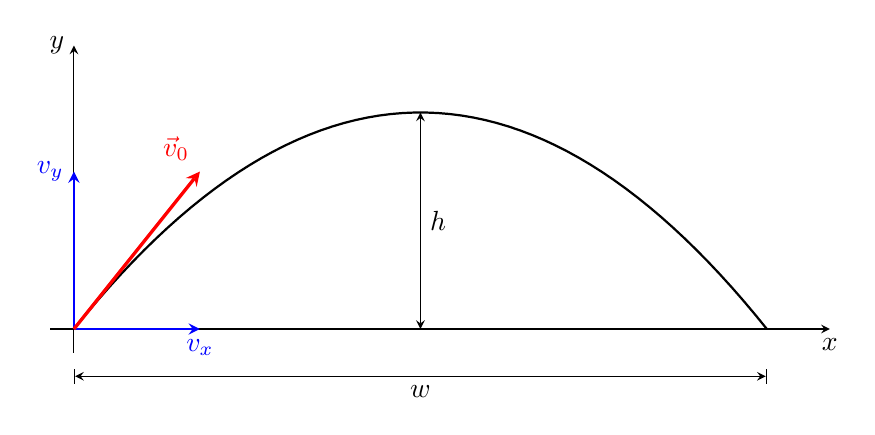
\begin{tikzpicture}[>=stealth]
 \draw[->] (-0.3,0) -- (9.6,0) node[below] {$x$};
 \draw[->] (0,-0.3) -- (0,3.6) node[left] {$y$};
 \draw[thick, domain=0:8.8, samples=60] plot (\x, {11*\x*(8.8-\x)/77.44});
 \draw[->, thick, blue] (0,0) -- (1.6,0) node[below] {$v_x$};
 \draw[->, thick, blue] (0,0) -- (0,2) node[left] {$v_y$};
 \draw[->, very thick, red] (0,0) -- (1.6,2) node[above left] {$\vec v_0$};
 \draw[<->] (4.4,0) -- (4.4,2.75) node[midway, right] {$h$};
 \draw[|<->|] (0,-0.6) -- (8.8,-0.6) node[midway, below] {$w$};
\end{tikzpicture}
\end{center}

Die beiden Teilbewegungen sind unabhängig: horizontal gleichförmig mit $v_x$, vertikal ein senkrechter Wurf mit $v_y$. Im höchsten Punkt ist die vertikale Geschwindigkeit null. Die Steigzeit folgt aus $0 = v_y - g\,t_\text{s}$:
\begin{align}
 t_\text{s} &= \tstF = \frac{\vy}{\gE} = \tst
\end{align}
Während des Steigens nimmt die vertikale Geschwindigkeit gleichmässig von $v_y$ auf null ab, die mittlere vertikale Geschwindigkeit ist also $v_y/2$. Damit ist die Wurfhöhe
\begin{align}
 h &= \frac{v_y}{2}\cdot t_\text{s} = \hmaxF \\
   &= \frac{\left(\vy\right)^2}{2\cdot\gE} \\
   &= \hmax \approx \result{\hmaxP{0}{2}}
\end{align}
Steigen und Fallen dauern gleich lang, die Flugzeit ist $2t_\text{s}$. In dieser Zeit fliegt der Ball horizontal
\begin{align}
 w &= v_x\cdot 2t_\text{s} = \xwF \\
   &= \frac{2\cdot\vx\cdot\vy}{\gE} \\
   &= \xw \approx \result{\xwP{0}{2}}
\end{align}
